\section{Configuration}
\label{sec:configuration}

The bot behaviour is ruled both by a \textit{local configuration} \textit{controller-specific configuration} loaded during botnet joining. The former is a fully customizable local YAML file, loaded during startup; the latter is given as a JSON response of \texttt{GET /init}, loaded when joining the botnet.
When no local configuration is specified, the bot looks for a YAML file named \texttt{config.yaml} in the present working directory. If not there, the bot loads the default configuration , which is hardly wired in code. For details about how to submit a custom configuration, please refer to \ref{sec:usage}.

We now show the configuration components, the YAML configuration schema to express them and a tool to generate configurations.

\begin{description}
  \setlength\itemsep{1em}

  \item[cnfInfo] if true, reports include the current bot configuration.

  \item[tgtInfo] if true, reports include details about the targets to attack.

  \item[sysInfo] if true, reports include details about the localhost system.

  \item[netInfo] if true, the bot report includes details about the network the localhost is attached to.

  \item[polling] period between consecutive requests to the controller for the next command to execute. The polling period is a random amount of time within a certain time interval. The randomness of period guarantees a greater variance in bots behaviour. Typically the period depends on the botnet needs. However, it is good practice not to set a too short period to ensure the concealment of the bot on the infected system\footnote{the default configuration provides a 10-15 seconds polling period for testing convenience.}.

  \item[reconnections] number of times the bot tries to connect to an unreacheable controller.

  \item[reconnectionWait] period between reconnections. The reconnection period is a random amount of time within a certain time interval. The period randomness guarantees a greater variance in bots behaviour. Such a period depends on the known controller availability.

  \item[proxy] HTTP proxy behind which the bot contacts remote controllers and targets. The default configuration has no proxy.

  \item[sleep] calendar for the sleeping mode. The default configuration has no sleep calendar.

  \item[authentication] a list of key-value pairs used as HTTP headers during bot-controller interactions. A minimal authentication setting should provide at least the \texttt{User-Agent}, but many more can be added, according to botnet security needs.

  \item[controllers] list of controllers to contact. The default configuration has an empty list of controllers. Each controller inherits (and may overwrite) the properties \texttt{polling, reconnections, reconnectionWait, proxy, sleep, authentication}.

\end{description}

The configuration is given in YAML format, with default values as comments. The schema shows some non primitive data types that deserves further attention.

\begin{verbatim}
  cnfInfo: True|False # True
  tgtInfo: True|False # True
  sysInfo: True|False # True
  netInfo: True|False # True
  polling: time-expression # 10-15:SECONDS
  reconnections: integer in [0,65535] # 0
  reconnectionWait: time-expression # 10-15:SECONDS
  proxy: proxy-expression # none
  sleep: cron-expression  # Null
  authentication: dict-object # {}
  controllers: [controller-object] # []
\end{verbatim}

A \texttt{time-expression} represents a temporal interval — e.g. a value in seconds between 3 and 5 seconds. This expression is a string in the form \texttt{min-max:unit}, where \texttt{min} is a positive long, \texttt{max} is a positive long greater than or equal to \texttt{min}, and \texttt{unit} is the string representation of a standard Java TimeUnit\footnote{i.e. NANOSECONDS, MICROSECONDS, MILLISECONDS, SECONDS, MINUTES, HOURS, DAYS.}. If \texttt{min} and \texttt{max} are both equal to a positive long \texttt{amount}, the time interval could be representaed both by the redundant expression \texttt{amount-amount:unit} and by the more compact expression \texttt{amount:unit}.

A \texttt{proxy-expression} represents a HTTP proxy — e.g. the proxy 123.123.123.123 with port 3000. This expression is a string in the form \texttt{address:port}, where \texttt{addres} is an IPv4 address and \texttt{port} is a port number. The expression can also be a string \texttt{none}, meaning that no proxy should be used, and \texttt{null}, meaning that any default proxy should be used.

A \texttt{cron-expression} represents a calendar — e.g. every Wednesday between 10 PM and 11PM. This expression is a standard Unix CRON expression. For details about the standard, please refer to \cite{cron-expression}.

A \texttt{dict-expression} represents a dictionary between strings and strings — e.g. "prop1" set to "val1".

A \texttt{controller-object} represents a bot controller — e.g. a controller with init interface X command interface Y and log interface Z. A controller is expressed in the following form:

\begin{verbatim}
  init: resource-expression
  cmd:  resource-expression
  log:  resource-expression
  polling: time-expression # 10-15:SECONDS
  reconnections: integer in [0,65535] # 0
  reconnectionWait: time-expression # 10-15:SECONDS
  proxy: proxy-expression # none
  sleep: cron-expression  # Null
  authentication: dict-object # {}
\end{verbatim}

where a \texttt{resource-expression} represents a readable local or remote resource — i.e. a standard file pathname or a remote Web URL.

\subsection{Sample configuration}
\label{sec:sample-configuration}

Here we show a sample configuration for reader's convenience. Other sample configurations can be found in \texttt{data/samples/configurations}.

\begin{verbatim}
  cnfInfo: True
  tgtInfo: False
  sysInfo: True
  netInfo: False
  polling: 10-15:SECONDS
  reconnections: 3
  reconnectionWait: 3-5:SECONDS
  proxy: 123.123.123.123:3000
  sleep: * * * SAT-SUN * ?
  authentication:
    User-Agent: MyAwesomeBot
    Authentication: Basic 123456789
    BotID: 270690
  controllers:
    - init: data/samples/controllers/1/botinit.json
      command: data/samples/controllers/1/botcmd.json
      log: data/samples/controllers/1/botlog.json
    - init: data/samples/controllers/2/botinit.json
      command: data/samples/controllers/2/botcmd.json
      log: data/samples/controllers/2/botlog.json
\end{verbatim}

\subsection{Configuration Dashboard}\label{sec:configuration-dashboard}
The Configuration Dashboard allows to generate the initialization YAML file for bot, as seen in the previous example. It is an intuitive web page with responsive design, that is automatically readapted to the device size from which is used. As we can see in Figure~\ref{fig:configuration-dashboard}, the first section of the Configuration Dashboard provides the chance to set to true or false the following fields: \textit{sysinfo}, \textit{netInfo}, \textit{cnfInfo} and \textit{tgtInfo}, enabling the appropriate checkbox. In the part below, we can act on polling and reconnection-wait values with a simple slider to establish the time interval within which the command operates. The reconnection box provides the opportunity to specify the number of connection attempts. The controllers table involves the insertion of a list of controllers, in where each controller group consists of: init, cmd, and log. Table’s fields can be, as already said, a path to a local file or a Web URL. Below, can be specified the default proxy and a set of authentication fields, defined with the pair: <\textit{field}, \textit{value}>. The last textbox allows to specify a regex with the desired sleepmode. A click on the "Generate Configuration" button lets you to generate the YAML configuration file for the bot. This file can be then copied to the clipboard, simply downloading them or submitting to the C\&C.

\begin{figure}[h]
  \centering
  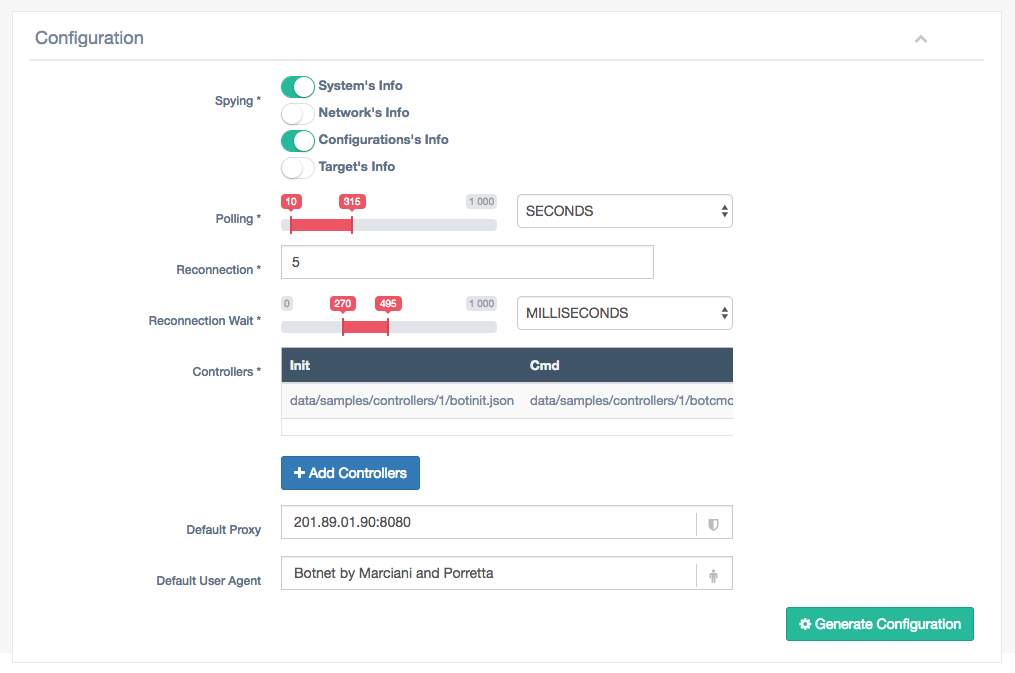
\includegraphics[scale=0.45]{./fig/configurationWUI.png}
  \caption{The dashboard to build \textit{local configuration}.}
    \label{fig:configuration-dashboard}
\end{figure}

\begin{figure}[h]
	\centering
	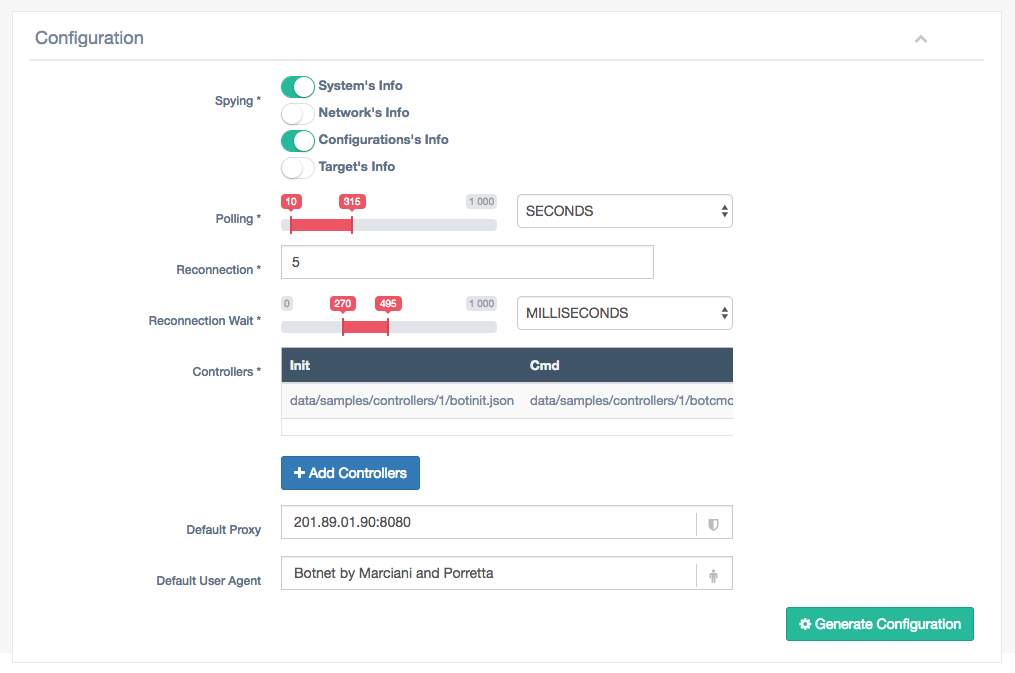
\includegraphics[scale=0.45]{./fig/configurationWUI.png}
	\caption{The dashboard to submit \textit{controller-specific} configuration.}
	\label{fig:initialization-dashboard}
\end{figure}
